%proprosed argument
I have designed an approach to these problems and have architected a straightforward solution that automates the steps described in the introduction. I hypothesize that Problem One is solved by the advent of combinatorial testing, which identifies most, if not all, of the test cases necessary for confidence in working software. My framework, Parmgen, has addressed the second problem, translating the English description of a test case into a concrete format that can be used as input into the program. I ask the user for a simple description of their input data, which requires less work than writing every data point by hand. Then I can use Python's random statistical distributions to generate those points and write them to a local file convenient for the tester's use. Figure \ref{fig:workflo} describes the user interaction with the architecture of tool. Red indicates user-written files. Blue indicates the output, the test data that can then be used for testing. This tool is written in the Python language, which is useful for prototyping the MVP (Minimum Viable Product). I call this entire pipeline GenSequence.

\begin{figure}[H]
\centering
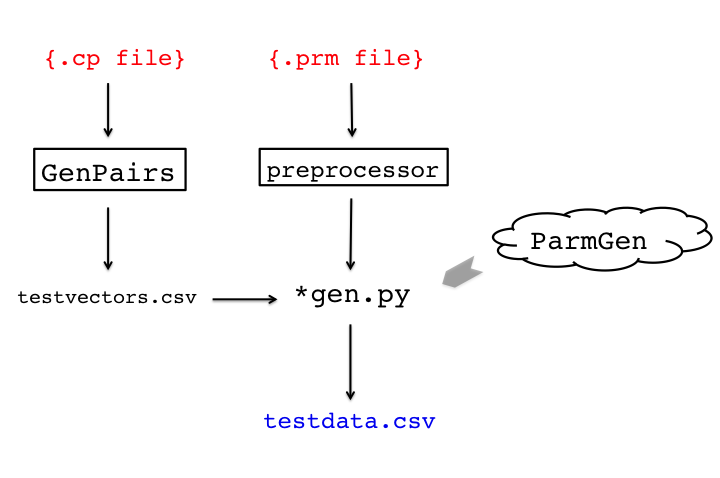
\includegraphics[scale=0.6]{workflow.png}
\caption{Basic Diagram of User's workflow with GenSequence}
\label{fig:workflo}
\end{figure}